\chapter{Background}
\section{Data Collection and Information Filtering}
\subsection{BigData}
The standards set by the World Wide Web consortium, formed in 1994, has led to large amounts of information sharing between the users and the hosts. As the users data grows, more hosts are required to sustain the growth. This growth can be viewed from the figure \autoref{fig:bigdata}.
\\
\begin{figure}[H]
	\centering
	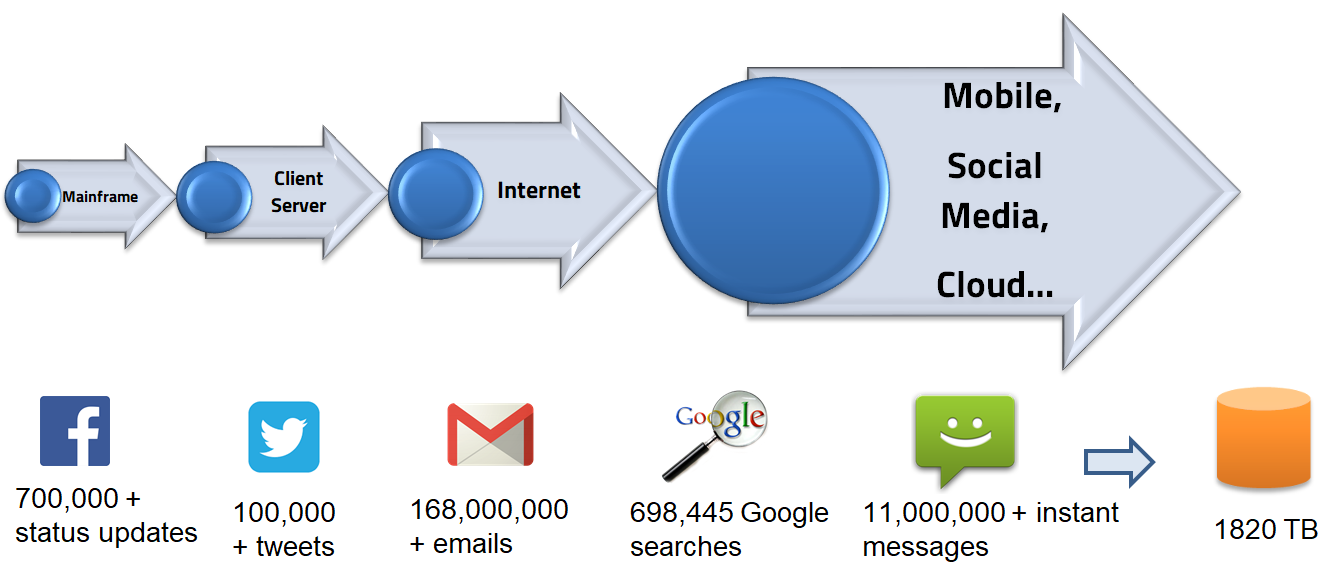
\includegraphics[width=0.7\linewidth]{bigdata}
	\caption{Growing Data Velocity per second}
	\label{fig:bigdata}
\end{figure}

\noindent To make any customer experience best, some of the ways recommendation technology is used to make it more personalize. These systems can perform well based on the large amount of data. Bigdata is a driving force behind recommendation engines.
To make this data useful, applications need to collect data, filter data in specific patterns from which we will get useful information. 

\subsection{Data Collection And Storage}

Data collection phase is foundation of accuracy of recommendation engine. It is helpful to generate user profile or model for the predictions. To well construct user profile, recommendation engine rely on different types of inputs such as explicit feedback which explicitly specified by user to notify user's interest in item or implicit feedback by understanding user preferences with user interaction with the system \cite{34}. 

\subsubsection{Explicit Data}
The application normally prompts the user through user interface to provide feedback about the product in order to understand user's preferences to improve model. User interacts with system by providing feedback. Explicit data is a information provided by user explicitly or \textbf{knowingly} in the form of ratings, reviews or comments. For example, \autoref{fig:explicit} shows that Netflix is collecting the data explicitly in the form of ratings given by user to different movies. 
\\

\begin{figure}[H]
	\centering
	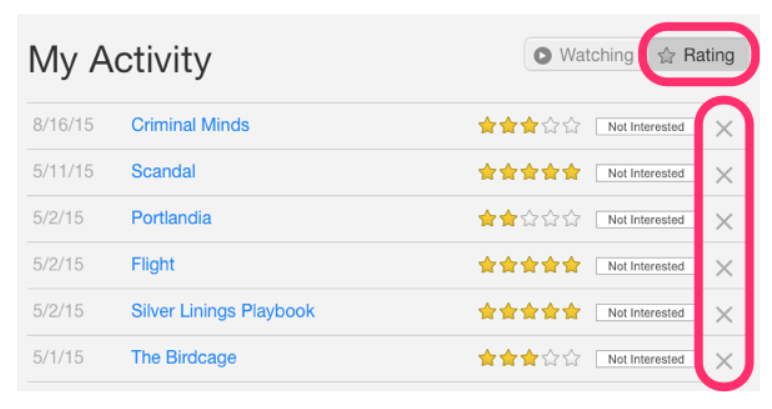
\includegraphics[width=0.9\linewidth]{explicit1}
	\caption{Explicit Data}
	\label{fig:explicit}
\end{figure}

Although explicit feedback requires more efforts from the user, it is still reliable data as it does not require any extraction of preferences and it maintains transparency into recommendation process \cite{35}. 
 
\subsubsection{Implicit Data}

The application tries to understand more about user's preferences by monitoring interactions of user such as browsing history, purchase history, button-clicks, links followed by user. Implicit data is a information provided by user \textbf{unknowingly} in the form of different interactions. For example, \autoref{fig:implicit} shows that Amazon is collecting the data implicitly in the form of storing user's order history. 
\begin{figure}[H]
	\centering
	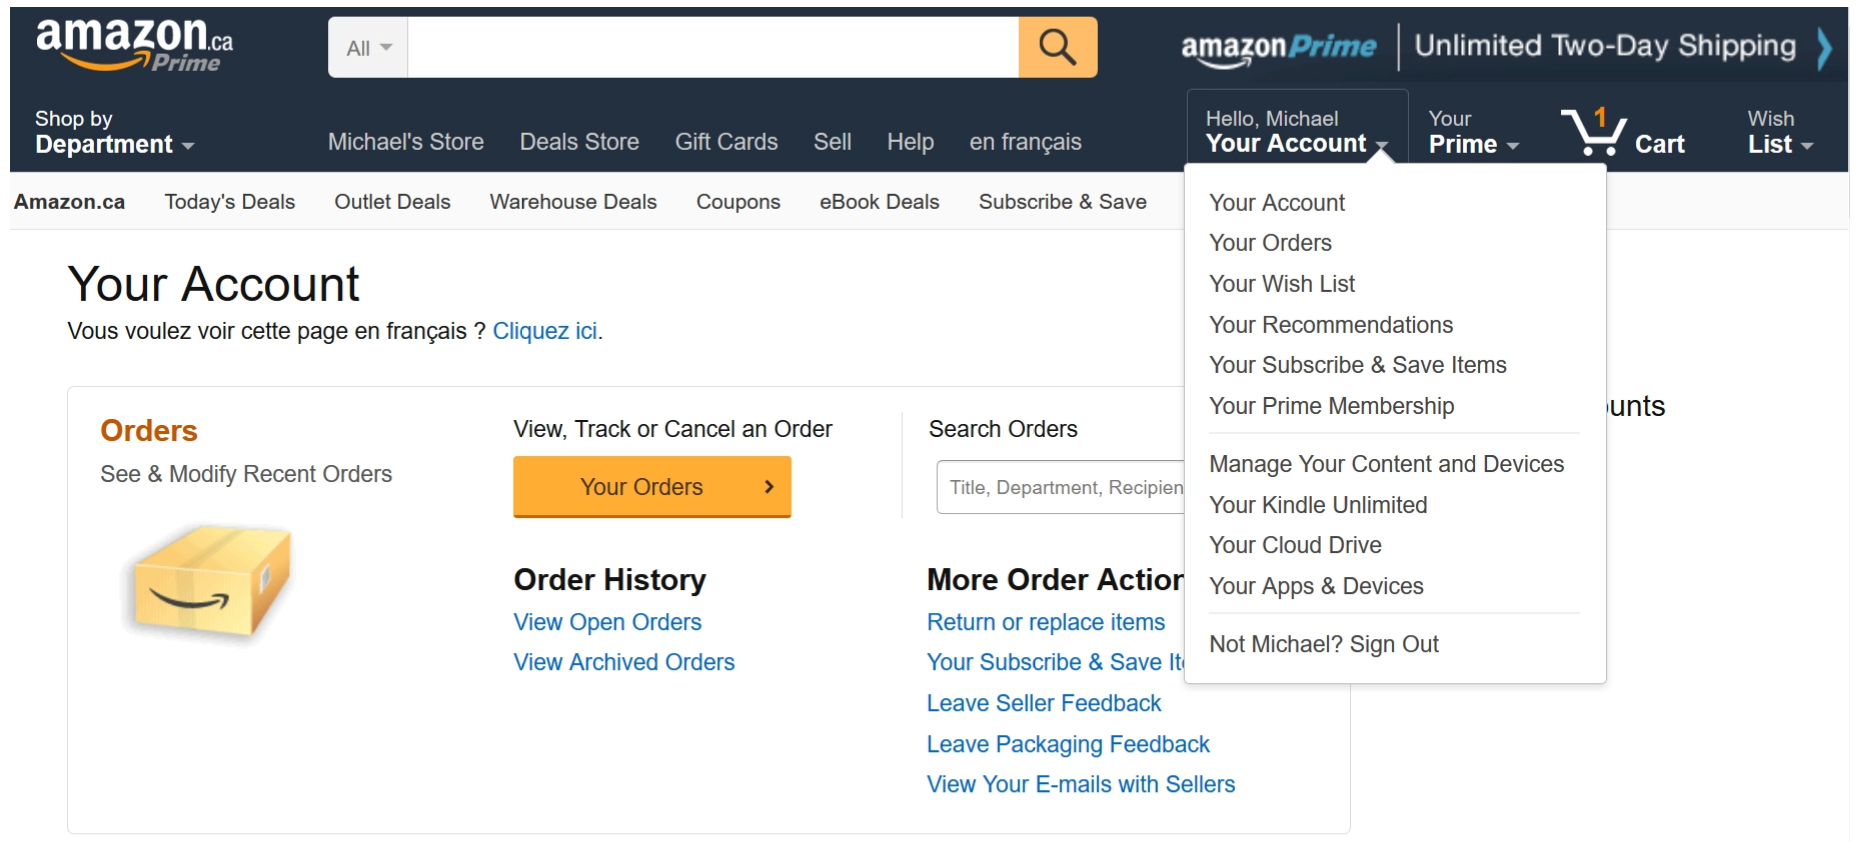
\includegraphics[width=0.9\linewidth]{implicit}
	\caption{Implicit Data}
	\label{fig:implicit}
\end{figure}

Although implicit feedback does not require more efforts from user, it is less accurate.\\

Explicit and implicit data collection methods are used for building online recommendation system. In this paper we are working on offline data. When we need to work on offline data, we need to gather data with different techniques. \\
Information Gathering involves web crawling, document processing, indexing and queryprocessing. A crawler processes all URLs via techniques like breadth-first search and depth-first search and stores the web servers response for each URL. The documents retrieved are then processed in order for its meta-data and to remove any noisy data. Data indexing is then applied so that retrieval and processing of extracted data is quicker.


\subsection{Information Filtering}

When a user requests information, it is treated as a query in the form of keywords and is applied on the indexed data. The objective of the query processor is to return most relevant documents to the user.

Filtering is a key component to retrieving adequate information per user preferences or user profile. User behavior is studied from past user profiles activities which helps to filter out any irrelevant data and provide apt suggestions pertaining to current needs. Part of information filtering that tries to predict a user's preference is known as a recommender system.